\documentclass[titlepage,a4paper]{article}

\usepackage[dutch]{babel}
\usepackage{graphicx}

\begin{document}
\title{Verslag Project Algoritmen en Datastructuren II Optimale binaire zoekbomen}
\author{Mathieu De Coster}
\date{26 november 2013}
\maketitle

\tableofcontents

\section{Bespreking van de verschillende implementaties}
Hieronder bespreek ik kort welke implementaties overeenkomen met welke klassen, en hoe ze presteren.

\subsection{Hulpklassen}
Om duplicatie van code te vermijden en bepaalde zaken te vereenvoudigen, heb ik een abstracte klasse AbstractBST toegevoegd die de interface BST implementeert. Deze klasse voorziet een wortel voor een boom en een printmethode die de boom uitprint naar standard output, maar ook twee methoden die de top met de kleinste sleutel (respectievelijk grootste) van twee toppen teruggeeft. De klasse bevat ook een implementatie voor balance en cost, die recursief werken.

Bovendien is er ook een abstracte klasse AbstractObst, die de klasse AbstractBST uitbreidt. Deze voorziet de methoden die gedeeld wordt door alle Obst bomen: getC, add en contains.

Ten slotte heb ik een Node klasse gemaakt, die een top voorstelt in een boom met een integer-waarde als sleutel. Deze klasse voorziet een methode om zichzelf en zijn kinderen naar standard output te printen. Een top houdt referenties naar zijn twee kinderen en zijn ouder bij.

\subsection{Zelforganiserende zoekbomen}
\subsubsection{Sbst1 - Semi-splay}
\paragraph{Implementatiedetails}
De klasse Sbst1 implementeert een semi-splay boom volgens de definitie uit de cursus.
Er wordt dus gesplayed na elke operatie: toevoegen en opzoeken.

Om bomen met zeer grote diepte te kunnen verwerken (en StackOverflows te vermijden) maak ik geen gebruik van recursie, maar van een while-loop in de add- en contains-methode, die zo diep in de boom kan gaan als nodig.

De splay-methode is een letterlijke implementatie van semi-splay in de cursus. Om eenvoudig de structuur van de vervangboom te bepalen, pas ik volgend trucje toe:

\begin{enumerate}
\item Het linkerkind is uiteraard het allerkleinste, dus \begin{verbatim}kleinste = min(min(top, ouder), grootouder)\end{verbatim}
\item Het rechterkind is het allergrootste, dus \begin{verbatim}grootste = max(max(top, ouder), grootouder)\end{verbatim}
\item De wortel is de middelste top. Hier zijn er twee gevallen mogelijk: de wortel is de grootste van het minimum of het kleinste van het maximum: \begin{verbatim}middel = max(min(top, ouder), grootouder)
if(middel == grootste || middel == kleinste)
    middel = min(max(top, ouder), grootouder)\end{verbatim}
\end{enumerate}

\paragraph{Correctheidstests}
De correctheid van de implementatie heb ik gecontroleerd door verschillende bomen met de hand op te bouwen volgens het algoritme uit de cursus, en de verschillende stappen te laten uitvoeren door mijn implementatie. Deze kwamen altijd overeen. Vervolgens heb ik ook sleutels toegevoegd die al in de boom zaten en sleutels opgezocht die niet in de boom zaten. Ook hierbij werd op een correcte manier gesplayed. Ik heb ook de return-waarden van de methoden add en contains gecontroleerd met de hand.

\paragraph{Tijdsmetingen en complexiteit}
Ik heb opeenvolgend bomen opgebouwd met $n$ elementen, waarbij $n$ varieert van 100.000 tot 5.000.000 in stappen van 100.000. Hierbij heb ik voor elke $n$ het algoritme 5 keer laten uitvoeren, en daarvan de gemiddelde tijd genomen.
Op een gelijkaardige manier heb ik de gemiddelde tijd voor de contains-methode berekend.
Tot slot heb ik ook bekeken of het splayen effici\"ent werkt door steeds hetzelfde element op te vragen in een zeer diepe boom en te kijken of het sneller gevonden werd.

Deze testcode bevindt zich in het bestand \emph{tests/TestSbst1.java}.

\begin{figure}[here]
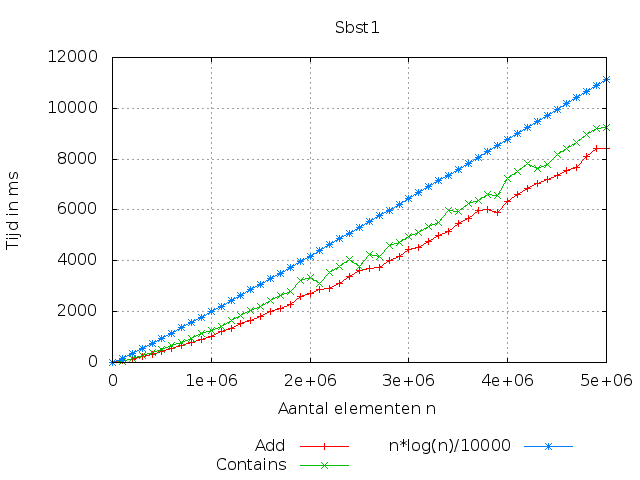
\includegraphics[width=0.9\linewidth]{../Resultaten/sbst1.png}
\caption{Tijdsmetingen van add en contains (semi-splay)}
\label{sbst1_add_contains}
\end{figure}

Uit Figuur \ref{sbst1_add_contains} leid ik af dat mijn implementatie een complexiteit van $O(log(n))$ per bewerking heeft; de geamortiseerde kost is dus $O(n*log(n))$ voor een reeks van n toevoegbewerkingen op een initieel lege semi-splayboom.
De grafiek toont namelijk dat de tijdsmetingen van mijn implementatie steeds kleiner zijn dan de grafiek van $O(\frac{n*log(n)}{1000})$, dus is dat een bovengrens voor de complexiteit.

\subsection{Gewone binaire zoekbomen}

\subsubsection{Obst1 - niet-geoptimaliseerde versie}
\paragraph{Implementatiedetails}
De klasse Obst1 is een implementatie van een gewone zoekboom. De add- en contains-methoden gebruiken net als bij Sbst1 geen recursie. De optimize methode gebruikt dynamisch programmeren.

De optimize methode werkt als volgt:

\begin{itemize}
\item Er worden eerst drie tweedimensionale arrays aangemaakt. Daarna wordt de boom in inorder doorlopen om een gesorteerde lijst van toppen te verkrijgen.

\item Vervolgens wordt het gewicht van elke deelboom T[i,j] berekend. Een boom T[i,i] is een enkele top, vandaar dat op de diagonaal gewoon de kost van die top staat. De rest van de elementen van de bovendriehoek in deze matrix worden berekend aan de hand van reeds ingevulde waarden.

\item Nu wordt de minimale kost van elke deelboom T[i,j] berekend. De hoofddiagonaal is opnieuw eenvoudig in te vullen. Andere waarden worden via de recursieve formule uit de opgave berekend, waarbij ik wel zorg dat we waarden geen tweemaal berekenen. Ik sla ook de wortel van de optimale deelboom op in een aparte matrix.

\item De optimale boom wordt heropgebouwd op een bottom-up manier, met behulp van een stapel.
\end{itemize}

\paragraph{Correctheidstests}
Om de correctheid te testen, vergelijk ik de inhoud van deze boom met die gemaakt in Sbst1. Ik vergelijk of dezelfde elementen er in zitten, en of ze evenveel elementen bevatten. Dit is het geval. Voor kleine bomen heb ik ze ook op papier uitgewerkt, en vergeleken met de implementatie. Daaruit bleek dat die voor de testgevallen correct werkt.

De optimize-methode heb ik met de hand gestest op papier, voor kleinere bomen. Ook nu bleek de correctheid.

\paragraph{Tijdsmetingen en complexiteit}
Uit Figuur \ref{obst_add_contains} blijkt dat ook toevoegbewerkingen en opzoekbewerkingen in een gewone binaire zoekboom een complexiteit hebben van $O(n*log(n))$. Dit hoeft niet te verbazen, aangezien het hier om willekeurige elementen gaat en er geen splay hoeft te worden toegepast.

\begin{figure}[here]
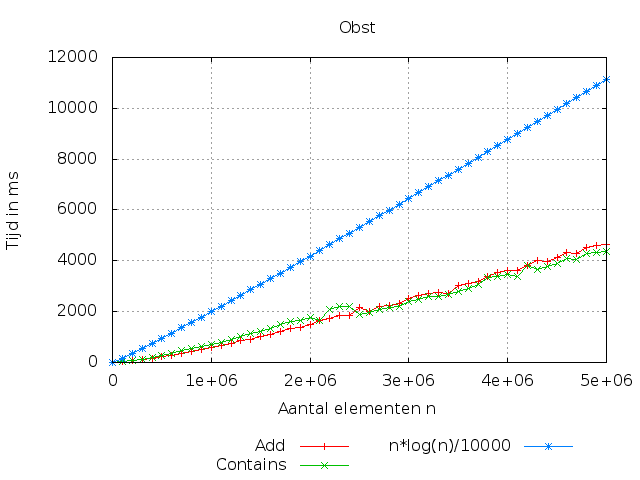
\includegraphics[width=0.9\linewidth]{../Resultaten/obst2.png}
\caption{Tijdsmetingen van add en contains (binaire zoekboom)}
\label{obst_add_contains}
\end{figure}

\textbf{TODO VERGELIJK ALS WE VAAK HETZELFDE ELEMENT OPZOEKEN OF TOEVOEGEN + BESPREKING OPTIMIZE}

In Figuur \ref{obst1_optimize} zien we dat de optimize-methode uit Obst1 in $O(n^3)$ draait. Dit is niet optimaal. Al voor zeer kleine $n$ is het niet meer mogelijk om de boom te optimaliseren binnen een redelijke tijd. Daarom heb ik gezocht naar een optimalisatie, die ik ge\"implementeerd heb ik Obst2.

\begin{figure}[here]
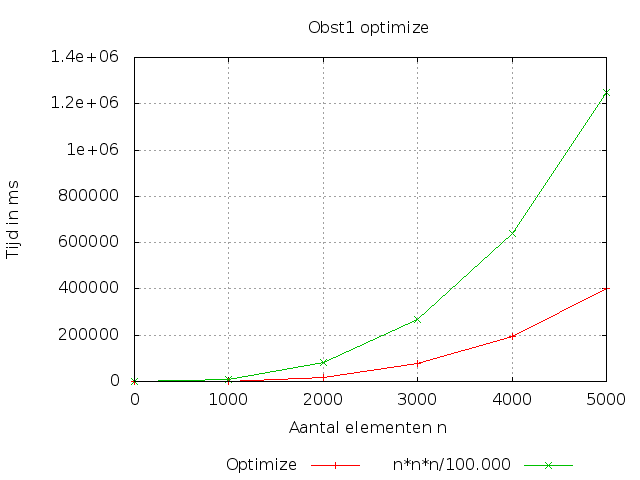
\includegraphics[width=0.9\linewidth]{../Resultaten/obst1_optimize.png}
\caption{Optimize in Obst1}
\label{obst1_optimize}
\end{figure}

\subsubsection{Obst2 - geoptimaliseerde versie}
\paragraph{Implementatiedetails}
Deze implementatie is volledig analoog aan die van Obst1, met een klein verschil bij het berekenen van de minimale kost. In Obst1 overlopen we alle mogelijke posities van de wortel \begin{verbatim}i <= k <= j\end{verbatim}
In deze implementatie doen we dat niet: \begin{verbatim}r[i][j-1] <= k <= r[i+1][j]\end{verbatim}

Hierbij is $k$ de index in de lijst van gesorteerde toppen: de top op index $k$ is dus de $k$-de kleinste top.

Dit vereist een beetje uitleg. In de eerste versie veronderstellen we dat de ideale wortel om het even welke top in de deelboom T[i,j] kan zijn. We weten echter al wat de ideale wortel is in de deelboom die bestaat uit kleinere toppen en grotere toppen. Aangezien de sleutel in deze wortel groter is dan de sleutel van de wortel in de linkerkinderdeelboom en kleiner dan die in de rechterkinderdeelboom, moeten we enkel $k$ beschouwen tussen deze twee waarden. Dit zorgt ervoor dat het aantal iteraties lus enorm verkleind kan worden. Stel bijvoorbeeld dat $i=0$ en $j=100$. Dan zijn er in de eerste versie 101 iteraties. In de tweede versie kan het zijn dat er slechts 2 zijn, als $r[i][j-1] == r[i+1][j]-1$.
\textbf{TODO TEKENING}

\paragraph{Correctheidstests}
De add- en contains-methoden zijn volledig hetzelfde als in Obst1, deze heb ik dus niet meer getest.

De optimize-methode heb ik getest door de uitvoer ervan te vergelijken met die van Obst1. Deze was hetzelfde voor alle testgevallen. Daaruit concludeer ik dat (als Obst1 inderdaad correct is) deze implementatie ook correct is.

\paragraph{Tijdsmetingen en complexiteit}
De enige methode die hier moet onderzocht worden is de optimize-methode. Deze blijkt heel wat sneller te werken dan die uit Obst1. Door enkele tests en een vergelijking kwam ik tot de volgende conclusie: de implementatie van optimize in Obst2 heeft een complexiteit van $O(n^2)$ in plaats van $O(n^3)$.

De tijdsmetingen van deze optimize methode zijn zichtbaar in Figuur \ref{obst2_optimize}. Een vergelijking tussen de twee volgt in de volgende sectie.

\begin{figure}[here]
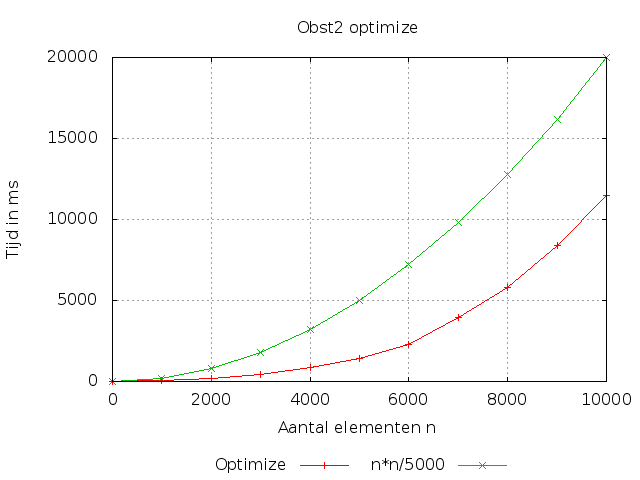
\includegraphics[width=0.9\linewidth]{../Resultaten/obst2_optimize.png}
\caption{Optimize in Obst2}
\label{obst2_optimize}
\end{figure}


\section{Vergelijkingen tussen verschillende zoekbomen}

\subsection{Sbst1 versus Obst: Add en contains}
Het leek me interessant om semi-splay te vergelijken met gewone zoekbomen. Daarom heb ik dezelfde reeks willekeurige elementen toegevoegd aan een Sbst1-boom en een Obst1-boom. De resultaten van deze tests zijn te zien in Figuur \ref{obst_add_contains_vs_sbst1}. Daaruit blijkt dat Obst1 beter presteert. Ik neem aan dat dit komt omdat deze boom niet moet splayen.

\begin{figure}[here]
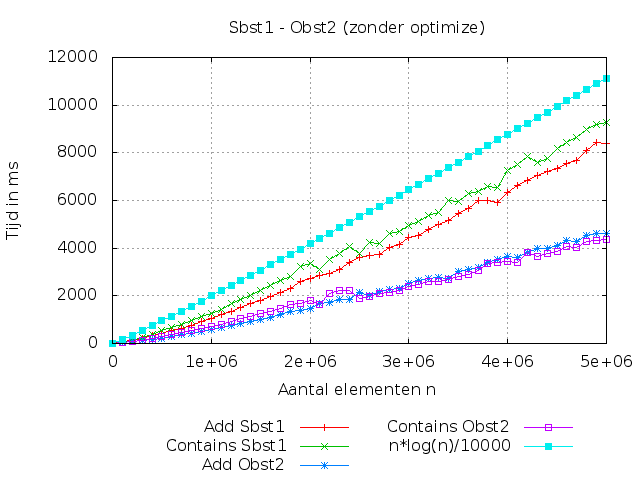
\includegraphics[width=0.9\linewidth]{../Resultaten/obst2_vs_sbst1.png}
\caption{Add en contains in een binaire zoekboom en in semi-splay}
\label{obst_add_contains_vs_sbst1}
\end{figure}

\subsection{Obst1 versus Obst2: Optimize}
Zoals hierboven vermeld is er een groot verschil in tijd tussen de optimize-methode van Obst1 en Obst2. In Figuur \ref{obst1_obst2_optimize} wordt dit aangetoond. Het betreft hier dezelfde tijdsmetingen als in de vorige secties, maar dan in dezelfde grafiek. Het valt snel op dat er een enorm verschil is in effici\"entie: de tijdsmetingen van Obst2 zijn haast niet zichtbaar.

\begin{figure}[here]
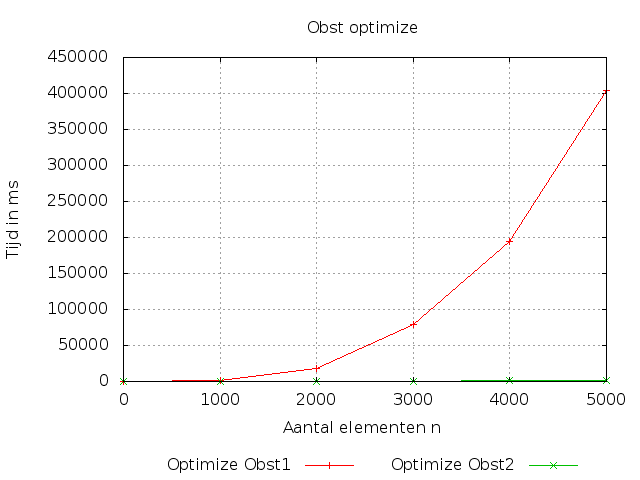
\includegraphics[width=0.9\linewidth]{../Resultaten/obst_optimize.png}
\caption{Obst1 versus Obst2: Optimize}
\label{obst1_obst2_optimize}
\end{figure}

\section{Theoretische vragen}
\subsection{Vraag 1}
Als we in de huidige implementatie een sleutel opzoeken die niet in de boom zit, moeten we altijd een heel pad doorlopen tot in de bladeren. Om dit effici\"enter te kunnen doen kunnen we dummy-toppen bijhouden. We zouden hiervoor de Node-klasse kunnen aanpassen zodat er een boolean waarde wordt bijgehouden die aangeeft of de top in de boom zit. Een dummy-top is dan een top waarbij deze op false staat. Voor de rest worden deze toppen beschouwd als gewone toppen. Als we bijvoorbeeld een dummy-top met sleutel $s$ hebben, en we willen $s$ toevoegen, moet de add-methode aangepast zijn zodat die de top met sleutel $s$ vindt en aanduidt dat die nu in de boom zit. De contains-methode moet ook rekening houden dat als de sleutel niet echt in de boom zit en dus een negatieve waarde teruggeven. 

Een voordeel van deze dummy-toppen: als de boom geoptimaliseerd wordt om een minimale kost te hebben, zal een zeer vaak opgezochte dummy-top ook naar boven verplaatst worden en dus effici\"enter kunnen worden opgezocht.

Dit heeft echter een nadelige invloed op de algemene effici\"entie van de boom. Er worden meer toppen bijgehouden, waardoor er meer vergelijkingen zijn bij toevoegen en opzoeken. Het balanceren en berekenen van de kost van de boom zal langer duren. Ten slotte zal dit vooral een negatieve invloed hebben op het optimize algoritme. De bottleneck is daar sowieso al het geheugen. Extra toppen toevoegen zal er voor zorgen dat de boom soms niet te optimaliseren is wegens gebrek aan geheugen.

\subsection{Vraag 2}
Aangezien een navigatie naar het linkerkind goedkoper is dan naar het rechterkind, willen we dit kunnen weergeven in het gewicht van een top. Omdat een vergelijking goedkoper is dan een opzoeking, willen we echter minder waarde hechten aan deze vergelijking. Om dit te bekomen kunnen we het gewicht van een opzoeking of toevoeging vermenigvuldigen met een bepaalde factor $k$. Als een top $t$ wordt opgezocht of toegevoegd, zal het gewicht van $t$ dus ge\"incrementeerd worden met $k$, bijvoorbeeld 2. Als er een navigatie naar een rechterkind wordt gedaan, wordt het gewicht verhoogd met 1. Hoe groter $k$, hoe minder belang we heffen aan de kost van het vergelijken van de sleutels. Zo wordt dus aangegeven dat als er in een top vaak genavigeerd wordt naar het rechterkind, deze navigaties duurder zijn. Als we dit op deze manier doen, moeten we niets aanpassen aan het berekenen van de kost van een boom.

\end{document}